\chapter{Theoretical Background}
\label{ch:Background}
In this chapter we define the necessary background for understanding PGExplainer as well as the follow-up work regarding its application on the Boolean Satisfiability Problem (SAT).

\section{Deep learning}
In this chapter we introduce Deep Learning (DL) in the context of Machine Learning (ML) and their concepts required for this work. The definitions in this chapter loosely follow Goodfellow et al.\cite{Goodfellow-et-al-2016}.

An ML algorithm generally learns to perform a certain task from data. Common ML tasks include classification, where the goal is to assign an input to one of $k$ categories, and regression, where the program shall predict a numeric value given some input. 

ML algorithms can be broadly divided into supervised and unsupervised learning. In this work, we focus on supervised learning, meaning that the algorithm learns from a dataset containing both features and labels or targets that the algorithm is supposed to predict. In other words, the algorithm learns from a training set of inputs $x$ and outputs $y$ to associate another unseen input with some output.

%Deep learning entails adding more layers and units to the model used in our algorithm to allow for representations of functions with increasing complexity.

DL entails expanding the size of the model used in our algorithm to allow for representations of functions with increasing complexity. This enables many human-solvable tasks that consist of mapping an input vector to an output vector to be performed with DL, given sufficiently large models and datasets.

In many cases DL involves optimizing a function, usually by minimizing $f(x)$. This objective function is also referred to as loss function in the context of minimization. %We denote $x^*=\text{arg min} f(x)$.
To minimize a function $f(x)$ we make use of the derivative $f'(x)$ that tells us how to change $x$ in order to get an improvement in $y$. We can reduce $f(x)$ by moving $x$ in the direction opposite of the sign of its derivative, since $f(x-\epsilon \text{ sign}(f'(x))) < f(x)$ for small enough $\epsilon$. This technique is called gradient descent (see Cauchy\cite{cauchy1847methode}).

Furthermore, a DL algorithm typically consists of the following components: a dataset specification, an objective function, an optimization procedure, like gradient descent, and a model. %5.10

\subsection{Multilayer Perceptron}
A classical DL model is the multilayer perceptron (MLP) with the general goal of approximating a function $f^*$. In the case of classification we could define a function $y = f^*(x)$ that maps an input $x$ to a label $y$. The MLP then defines the mapping $y = f(x;\Theta)$ and learns the value of the parameters $\Theta$ that best approximate the function. These models are also referred to as feedforward neural networks, as they process information from $x$, through the intermediate computations that define $f$, to the output $y$ without feedback connections that would feed outputs back to itself. The name network is derived from their representation as a composition of multiple different functions, that are described by a directed acyclic graph. An example network is $f(x) = f^{(3)}(f^{(2)}(f^{(1)}(x)))$ that consists of input layer $f^{(1)}$, hidden layer $f^{(2)}$ and output layer $f^{(3)}$. The length of this chain of functions is called depth and origin of the term "deep learning". The approximation is achieved by training our network with training data, that consists of approximated examples of $f^*(x)$ at different points in the training and labels $y\approx f^*(x)$. These training examples dictate the output layer to generate a value close to $y$ for each $x$. The learning algorithm then learns to utilize the other hidden layers, without specified behaviors, to achieve the best approximation. It is to note that the hidden layers are vector-valued with each vector element, referred to as unit, loosely taking the role of a neuron in neuroscience. Models are therefore also referred to as neural networks.

%We use non-linear activation functions in layers to describe features and keep the model from learning a strictly linear transformation of its inputs. Result for a layer is vector of hidden units $h=g(W^Tx+b)$, where $W$ contains the weights of a linear transformation and b the biases. x is the input vector. $g$ is the activation function that is usually applied element-wise, such as ReLU or Sigmoid.

A linear layer for our model with parameters $\Theta$ consisting of weight $w$ and bias $b$ can be described as $f(x; w,b)=x^Tw+b$ for an input vector $x$. To keep the model from strictly learning a linear function of its inputs we can calculate the values of a layer $h$ by applying an activation function $g$ to its output to describe the features. This results in our hidden layer $h=g(W^Tx+c)$, with $W$ containing the weights of a linear transformation and $c$ the biases.

The activation function usually serves the purpose of mapping to a real number between $0$ and $1$, imitating the activation of a neuron. We try to use activation functions that are continuous differentiable and easily calculated, to minimize computational complexity (see Liu et al.\cite{Liu2020}). Examples are the Sigmoid function

%GNN BOOK: \\
%initiated with random weights or values, updated in each neuron with backpropagation. Learned knowledge stored in connections digitally. \\
%Each neuron therefore takes inputs $x_1, ..., x_n$ with corresponding weights $w_1, ..., w_n$ and an offset $b$. A layer can then be described as a linear function $y=\sum_{i=1}^{n} w_i x_i +b$ that is optionally passed through a non-linear activation function $f$ that generates the output of the current layer $z = f(y)$. The activation function usually serves the purpose of mapping to a real number between $0$ and $1$, imitating the activation of a neuron. We try to use activation functions that are continuous differentiable and easily calculated, to minimize computational complexity. Examples are the Sigmoid function 
\begin{equation}
    \sigma (x)= \frac{1}{1+e^{-x}}
\end{equation}
and the Rectified Linear Unit (ReLU)
\begin{equation}
    ReLU(x)=\begin{cases}
        0 & x \leq 0, \\
        1 & x > 0.
    \end{cases}
\end{equation}


%To minimize a function $f(x)$ we make use of the derivative $f'(x)$ that tells us how to change $x$ in order to get an improvement in $y$. We can reduce $f(x)$ by moving $x$ in the direction opposite of the sign of its derivative, since $f(x-\epsilon \text{sign}(f'(x))) < f(x)$ for small enough $\epsilon$. This technique is called gradient descent (see Cauchy\cite{cauchy1847methode}).

\subsection{Backpropagation}
The back propagation algorithm is commonly used during neural network training. It optimizes the network parameters by leveraging gradient descent. It first calculates the values for each unit in the network given the input and a set of parameters in a forward order. Then the error for each variable to be optimized is calculated, and the parameters are updated according to their corresponding partial derivative backwards. These two steps will repeat until reaching the optimization target. \\
TODO: Concrete formulas with chain rule of calculus? 

\subsection{TODO: Regularization}
"A central problem in machine learning is how to make an algorithm that will
perform well not just on the training data, but also on new inputs. Many strategies
used in machine learning are explicitly designed to reduce the test error, possibly
at the expense of increased training error. These strategies are known collectively
as regularization."

Parameter Norm Penalties (e.g. Weight decay)
%"Many regularization approaches are based on limiting the capacity of models, such as neural networks, linear regression, or logistic regression, by adding a parameter norm penalty Ω(θ) to the objective function J. We denote the regularized objective function by ˜ J: J˜(θ; X, y) = J(θ; X, y) + αΩ(θ)
%where α ∈ [0, ∞) is a hyperparameter that weights the relative contribution of the norm penalty term, Ω, relative to the standard objective function J. Setting α to 0 results in no regularization. Larger values of α correspond to more regularization. When our training algorithm minimizes the regularized objective function J˜ it will decrease both the original objective J on the training data and some measure of the size of the parameters θ (or some subset of the parameters). Different choices for the parameter norm Ω can result in different solutions being preferred. In this section, we discuss the effects of the various norms when used as penalties on the model parameters." e.g. L1 or L2 norm

Early stopping
"When training large models with sufficient representational capacity to overfit
the task, we often observe that training error decreases steadily over time, but
validation set error begins to rise again."
"This means we can obtain a model with better validation set error (and thus,
hopefully better test set error) by returning to the parameter setting at the point in
time with the lowest validation set error."
"Every time the error on the validation set
improves, we store a copy of the model parameters. When the training algorithm
terminates, we return these parameters, rather than the latest parameters."
"algorithm terminates when no parameters have improved over the best recorded
validation error for some pre-specified number of iterations. "

Dropout

\subsection{Batch Normalization}
In deep models composed of several layers the gradient tells us how to update each parameter assuming that the other layers do not change. Since in practice all layers are updated simultaneously, this may lead to unexpected results. Batch normalization is an optimization technique that can be applied to any input or hidden layer to reduce the aforementioned problem\cite{Goodfellow-et-al-2016}.

Let $\mathbf{B}$ be a minibatch of activations of the layer to normalize, in the form of a design matrix with rows of activations. To normalize $\mathbf{B}$, it is replaced by
\begin{equation}
    \mathbf{B}' = \frac{\mathbf{B} - \boldsymbol{\mu}}{\boldsymbol{\sigma}},
\end{equation}
where $\boldsymbol{\mu}$ is a vector containing the mean of each unit and $\boldsymbol{\sigma}$ is a vector containing the standard deviation of each unit. Each activation is normalized individually with the $\boldsymbol{\mu}$ and $\boldsymbol{\sigma}$ corresponding to its row. The network processes $\mathbf{B}'$ as functionally equivalent to $\mathbf{B}$. During training,
\begin{equation}
    \boldsymbol{\mu} = \frac{1}{m}\sum_i \mathbf{B}_i
\end{equation}
and
\begin{equation}
    \boldsymbol{\sigma} = \sqrt{\delta + \frac{1}{m} \sum_i (\mathbf{B}_i - \boldsymbol{\mu})^2},
\end{equation}

where $\delta$ is a small positive value introduced to avoid $\sqrt{z}$ at $z = 0$ and $m$ is the number of elements in the batch. It is important to note that back propagation is performed through all three operations, to prevent the gradient from proposing an operation that solely increases the mean and standard deviation of the output of a layer. Batch normalization therefore reparameterizes the model to include some units that are standardized by definition.

When testing the model, we replace $\boldsymbol{\mu}$ and $\boldsymbol{\sigma}$ with running averages that were collected during training, to enable the evaluation of individual examples outside minibatches.

\subsection{Monte Carlo Sampling}
In order to best approximate a randomized algorithm we can make use of Monte Carlo methods as described in Goodfellow et al.\cite{Goodfellow-et-al-2016}[p.590]. A common practice in ML is to draw samples from a probability distribution and using these to form a Monte Carlo estimate of some quantity. This can be used to train a model that can then sample from a probability distribution itself. \\
More specifically, the idea of Monte Carlo sampling is to view a sum as if it was an expectation under some distribution and to approximate this estimate with a corresponding average.
Let 
\begin{equation}
    s = \sum_x p(x)f(x)=E_p[f(x)]
\end{equation}
be the sum to estimate with $p$ being a probability distribution over a random variable $x$. Then $s$ can be approximated by drawing $n$ samples from $p$ and constructing the empirical average 
\begin{equation}
    \hat{s}_n=\frac{1}{n}\sum_{i=1}^n f(x^{(i)}).
\end{equation}


\section{Graph Theory}
These definitions will loosely follow Liu et al.\cite{Liu2020}. A graph is a data structure consisting of a set of nodes that are connected via edges, modeling objects and their relationships. It can be represented as $G=(V,E)$ with $V=\{v_1,v_2...v_n\}$ being the set of $n$ nodes, and $E \in V \times V$ the set of edges. We adopt the conventions from Diestel\cite{Diestel2017}[p.2] to refer to the node and edges set of any graph $G$ with $V(G)$ and $E(G)$ respectively, regardless of the actual names of the sets, as well as a referring to $G$ with node set $V$ as $G$ on $V$. An edge $e=(u,v)$, sometimes accompanied by an edge weight $e_{u,v}\in (0,1)$, connects nodes $u$ and $v$, making them neighbors. The neighborhood $\mathcal{N}(u)$ of node $u$ in $V(G)$ is defined as $\mathcal{N}(u) = \{v \in V(G) \mid (v,u) \in E(G)\}$. We define the $k$-hop neighborhood of node $u$ in $V(G)$ as $\mathcal{N}_k(u) = \{v \in V(G) \mid dis_G(v,u) \leq k\}$, where $dis_G(v,u)$ denotes the distance of nodes $v, u$ in $G$, defined as the length of the shortest path between the two nodes. Edges are either directed or undirected and lead to directed or undirected graphs if exclusively present. The degree of a node $v$ is the number of edges connected to $v$ and denoted by $d(v)$. $G$ can be described by an adjacency matrix $A \in \mathbb{R}^{n \times n}$, where

Nodes in V are associated with the d-dimensional
features, denoted by X RN d
\begin{equation*}
    A_{ij}=\begin{cases}
        1 & \text{if } \{v_i,v_j\}\in E \text{ and } i \neq j, \\
        0 & \text{otherwise.}
    \end{cases}
\end{equation*}
If $G$ is an undirected Graph the adjacency matrix will be symmetrical. \\
Alternatively an undirected graph $ G=(V, E)$ with $n$ nodes and $m$ edges can be represented as an incidence matrix $M \in \mathbb{R}^{n \times m}$, where
\begin{equation*}
    M_{ij}=\begin{cases}
        1 & \text{if } \exists k \text{ s.t. } e_j = \{v_j, v_k\}, \\
        0 & \text{otherwise.}
    \end{cases}
\end{equation*}
The diagonal degree matrix $D\in \mathbb{R}^{n\times n}$ of $G$ is defined via:
\begin{equation*}
    D_{ii} = d(v_i).
\end{equation*}

$G$ is called a subgraph of another graph $G'=(V',E')$ if $V(G) \subseteq V(G')$ and $E(G) \subseteq E(G')$. This is denoted as $H \subseteq G$. The number of nodes in a graph $|V|$ is its order and the number of edges $|E|$ is its size (see Diestel\cite{Diestel2017}).
We additionally define bipartite graphs according to Asratian et al.\cite{asratian1998}: A graph $G$ is bipartite if the set of nodes $V$ can be partitioned into two sets $V_1$ and $V_2$ so that no two nodes from the same set are adjacent. The sets $V_1$ and $V_2$ are called colour classes and $(V_1, V_2)$ is a bipartition of $G$. This means that if a graph is bipartite all nodes in $V$ can be coloured by at most two colours so that no two adjacent nodes share the same colour.\\
\begin{figure}[h]
    \centering
    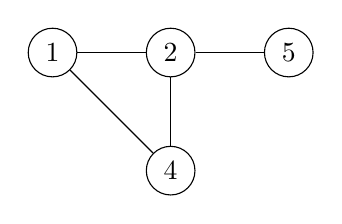
\begin{tikzpicture}[node distance=1.5cm, every node/.style={draw, circle}]
        % Define Nodes
        \node (1) {1};
        \node (2) [right of=1] {2};
        \node (4) [below of=2] {4};
        \node (5) [right of=2] {5};
        
        % Draw Edges
        \draw (1) -- (2);
        \draw (2) -- (4);
        \draw (1) -- (4);
        \draw (2) -- (5);
    \end{tikzpicture}
    \caption{A simple undirected graph $G$ with $V=\{1,2,4,5\}$ and $E=\{\{1,2\},\{2,4\},\{1,4\},\{2,5\}\}$.}
    \label{fig:graph-example}
\end{figure}

\textbf{Random Graphs}
\label{sec:random-graphs}

%Gilbert\cite{} describes the process of generating a random graph of order $N$ by assigning a common probability to exist in the graph to each potential edge between two nodes. Note that these random selections are made independently of each other, effectively drawing from a Bernoulli distribution. \\
Gilbert\cite{gilbert1959random} describes the process of generating a random graph of order $N$ by assigning a common probability of existence to each potential edge between any two nodes. For each of these potential edges an experiment is performed independently to determine whether it shall be included in the resulting graph. Note that this process can be modeled using a Bernoulli distribution.
%The actual edges in the graph are then selected by performing random experiments, made independently of each other, and can therefore be described by a Bernoulli distribution.
%Note that these random selections are made independently of each other and effectively drawn from a Bernoulli distribution.

%Version 1 (probability space for PGE not needed, definition for one random graph suffices?): \\
A random graph is further described by Diestel\cite{Diestel2017}[p.323] as follows. Let $V = \{0,...,n-1\}$ be a fixed set of $n$ elements. Say we want to define the set $\mathcal{G}$ of all graphs on $V$ as a probability space, which allows us to ask whether a Graph $G \in \mathcal{G}$ has a certain property. To generate our random graph we then decide from some random experiment whether $e$ shall be an edge of $G$ for each potential $e \in V \times V$. The probability of success - accepting $e$ as edge in $G$ - is defined as $p \in [0,1]$ for each experiment. This leads to the probability of $G$ being a particular graph $G_0$ on $V$ with e.g. $m$ edges being equal to $p^m q^{\binom{n}{2}-m}$ with $q:=1-p$.
\bigskip

%Version 2: \\
%A random graph is further described by Diestel\cite{Diestel2017}[p.323] as follows. Let $V = \{0,...,n-1\}$ be a fixed set of $n$ elements. To generate our random graph we then decide from some random experiment whether $e$ shall be an edge of $G$ for each potential $e \in V \times V$. The probability of success - accepting $e$ as edge in $G$ - is defined as $p \in [0,1]$ for each experiment. This leads to the probability of $G$ being a particular graph $G_0$ on $V$ with e.g. $m$ edges being equal to $p^m q^{\binom{n}{2}-m}$ with $q:=1-p$. It follows our desired probability space $\mathcal{G}=(n,p)$ as the product space
%\begin{equation}
%    \Omega := \prod_{e \in [V]^2} \Omega_e
%\end{equation}
%with $\Omega_e := \{0_e,1_e\}$, $\mathbb{P}_e(\{1_e\}) := p$ and $\mathbb{P}_e(\{0_e\}) := q$.
%TODO: This is probably unnecessary for PGE.
%\begin{equation}
%    E(G) = \{e | \omega(e) = 1_e\}
%\end{equation}
%E(G) = Edges of G. G is called a random graph on V with edge probability $p$. \bigskip

\section{Information Theory}
To fully understand the learning objective of PGExplainer it is necessary to define the concepts of entropy and mutual information. We follow the definitions by Cover et al.\cite{Cover2005}[p.13] if not stated otherwise.

\subsection{Entropy}
%TODO: REVISE THIS. Probably best to define with general expactation, for continous and discrete, according to Goodfellow. Derive conditional entropy for general case. Only apply discrete case where needed? (cross entropy in PGE) \bigskip

Entropy is used to describe the uncertainty of a random variable. It measures the amount of information required on average to describe a random variable. Let $X$ be a discrete random variable with alphabet $\mathcal{X}$ and probability mass function $p(x)=Pr\{X=x\}$ for $x\in X$.
The entropy $H(X)$, also written as $H(p)$, is defined as
\begin{equation}
    H(X) = -\sum_{x \in \mathcal{X}} p(x) \log p(x).
\end{equation}
%TODO: WE USE NATURAL LOGARITHM IN CODE!
The log is to the base $e$ and entropy is measured in nats in our case. TODO: DEFINE EDGE CASES log 0 %A simple example is tossing two coins: There are four possible outcomes $\mathcal{X}=\{00,10,01,11\}$, 0 for heads and 1 for tails, each with a probability $p=0,25$. The resulting entropy $H(X)=2$ represents that two bits of information can be stored this way. \bigskip
\\
%TODO: DIFFER MORE CLEARLY FROM CROSS? \\
%Analogously we define the joint entropy $H(X,Y)$ of a pair of discrete random variables $(X,Y)$ with a joint distribution $p(x,y)$ as follows:
%\begin{equation}
%    H(X,Y)=-\sum_{x \in \mathcal{X}} \sum_{y \in \mathcal{Y}} p(x,y) \log p(x,y).
%\end{equation}
The conditional entropy of $Y$ given $X$ is defined as the expected value of the entropies of the conditional distributions, averaged over the conditioning random variable. If $(X,Y) \sim p(x,y)$ for a pair of discrete random variables $(X,Y)$ with joint distribution $p(x,y)$, the conditional entropy is defined as
\begin{align}
    H(Y|X)&= -\sum_{x \in \mathcal{X}} p(x) H(Y|X=x) \\
    &= - \sum_{x \in \mathcal{X}} \sum_{y \in \mathcal{Y}}p(x,y) \log p(y|x) \\
    &= -\mathbb{E} \log p(Y|X),
\end{align}
with expectation $\mathbb{E}$.

\subsection{Relative Entropy and Cross-Entropy}
%Elements of Information Theory: equation 2.26 describes KL distance/relative entropy \bigskip
The relative entropy between two distributions is a measure of "distance" between the two. It measures the inefficiency of assuming a distribution to be $q$ when the true distribution is $p$. It is not a true measure of distance as it is among other things not symmetrical. The relative entropy takes a value of $0$ only if $p = q$.
We define the KL divergence or relative entropy between two probability mass functions $p(x), q(x)$ as
\begin{equation}
    D_{KL}(p||q) = \sum_{x \in \mathcal{X}} p(x)\log \frac{p(x)}{q(x)}
\end{equation}
Suppose we know the true distribution $p$ of our random variable. We could then construct a code with an average description length of $H(p)$. If we used the code for the distribution $q$ instead, we would need $H(p) + D_{KL}(p||q)$ nats to describe the random variable on average. This is also referred to as the cross-entropy (see Goodfellow et al.\cite{Goodfellow-et-al-2016}[p.74]):
\begin{equation}
    H(p,q) =  H(p) + D_{KL}(p||q)
\end{equation}


%The following definitions loosely follow Goodfellow et al.\cite{Goodfellow-et-al-2016}[p.74].
%The relative entropy is a measure of the distance between two distributions.
%"measure how different these two distributions are" \cite{Goodfellow-et-al-2016}
%"In the case of discrete variables, it is the extra amount of information needed to send a message containing symbols drawn from probability distribution P, when we use a code that was designed to minimize the length of messages drawn from probability distribution Q."
%"The KL divergence is 0 if and only if P and Q are the same distribution in the case of discrete variables"
%non symmetrical.
%"When computing many of these quantities, it is common to encounter expressions of the form 0 log 0. By convention, in the context of information theory, we treat these expressions as limx→0 x log x = 0. \\
%We define the KL divergence or relative entropy between two probability distributions $P, Q$ as
%\begin{equation}
%    D_{KL}(P||Q) = \sum_{x \in \mathcal{X}} P(x)\log \frac{P(x)}{Q(x)}
%\end{equation}

%The cross entropy is closely related to KL distance and therefore defined as
%\begin{align}
%    H(P,Q) &= -\mathbb{E}_{x\sim P}\log Q(x) \\
%    &= H(P) + D_{KL}(P||Q)
%\end{align}

We derive for the discrete case with mass probability functions $p, q$ defined on the same support $\mathcal{X}$:
\begin{align}
    H(p,q) = H(p) + D_{KL}(p||q) &= -\sum_{x \in \mathcal{X}} p(x) \log p(x) + \sum_{x \in \mathcal{X}} p(x)\log \frac{p(x)}{q(x)} \\
    &= -\sum_{x \in \mathcal{X}} p(x) \log p(x) + \sum_{x \in \mathcal{X}} p(x) \log p(x) -\sum_{x \in \mathcal{X}} p(x) \log q(x) \\
    &= -\sum_{x \in \mathcal{X}} p(x) \log q(x)
\end{align}

\subsection{Mutual Information}
%(see Cover et al.\cite{Cover2005}[p.19])
Another closely related concept is mutual information. It measures the amount of information that one random variable contains about another or the reduction in uncertainty of said variable due to knowing the other. A high mutual information therefore implies that the information of one variable can be gathered from the other.

Let $X$ and $Y$ be two random variables with the joint probability mass function $p(x,y)$ and marginal probability mass functions $p(x)$ and $p(y)$. Mutual information $I(X;Y)$ is the relative entropy between the joint distribution and the product distribution $p(x)p(y)$: 
\begin{align}
    I(X;Y)&=\sum_{x \in \mathcal{X}}\sum_{y \in \mathcal{Y}} p(x,y)\log \frac{p(x,y)}{p(x)p(y)} \\
    &= H(X) - H(X|Y)
\end{align}

\section{Graph Neural Networks}
TODO: DOES THIS CONVEY MESSAGE PASSING???

Graph Neural Networks(GNNs)\cite{4700287} are a DL-based approach that operates on graphs. Due to their unique non-Euclidean property, they find usage in classification, link prediction, and clustering tasks. Their high interpretability and strong performance have led to GNNs becoming a commonly employed method in graph analysis. They combine the key features of convolutional neural networks\cite{726791}, such as local connection, shared weights, and multi-layer usage, with the concept of graph embeddings\cite{cai2018comprehensive} (TODO: NON-EXISTENT?) to leverage the power of feature extraction and representation as low-dimensional vectors for graphs (see Liu et al.\cite{Liu2020}).\bigskip

Graphs are a common way of representing data in many different fields, including ML. ML applications on graphs can mostly be divided into graph-focused tasks and node-focused tasks. For graph-focused applications our model does not consider specific singular nodes, but rather implements a classifier on complete graphs. In node-focused applications however the model is dependent on specific nodes, leading to classification tasks that rely on the properties of each node.
The supervised GNN model by Scarselli et a.\cite{4700287} tries to preserve the important,  structural information of graphs by encoding their topological relationships among nodes.

A node is naturally defined by its features as well as its related notes in the graph. The goal of a GNN is to learn state embeddings $\mathbf{h}_v \in \mathbb{R}^S$ for each node $v$, that map the neighborhood of a node into a representation. These embeddings are used to obtain outputs $\mathbf{o}_v$, that e.g. may contain the distribution of a predicted node label. The GNN model proposed by Scarselli et al.\cite{4700287} uses undirected homogeneous graphs with $\mathbf{x}_v$ describing the $d$-dimensional features of each node and $x_e$ the optional features of each edge. $co[v]$ and $ne[v]$ denote the set of edges and neighbors of node $v$ respectively. The model updates the node states according to the input neighborhood with a local transition function $f$ that is shared by all nodes. Additionally, the local output function $g$ is used to produce the output of each node. $\mathbf{h}_v$ and $\mathbf{o}_v$ are therefore defined as
\begin{equation}
    \mathbf{h}_v = f(\mathbf{x}_v, \mathbf{x}_{co[v]}, \mathbf{h}_{ne[v]}, \mathbf{x}_{ne[v]}),
    \label{eq:gnn_state_local}
\end{equation}
\begin{equation}
    \mathbf{o}_v = g(\mathbf{h}_v, \mathbf{x}_v),
\end{equation}
with $\mathbf{x}$ denoting input features and $\mathbf{h}$ the hidden state. $\mathbf{x}_v, \mathbf{x}_{co[v]}, \mathbf{h}_{ne[v]}, \mathbf{x}_{ne[v]}$ denote the features of the node $v$ and of its edges, as well as the states and features of its neighboring nodes, respectively. We define $\mathbf{H}, \mathbf{O}, \mathbf{X} \text{ and  }\mathbf{X}_N$ as the matrices that are constructed by stacking all states, outputs, features, and node features, respectively. This allows us to define with the global transition function $F$ and the global output function $G$, which are stacked versions of their local equivalent for all nodes in a graph: 
\begin{equation}
    \mathbf{H} = F(\mathbf{H}, \mathbf{X}),
    \label{eq:gnn_state_global}
\end{equation}
\begin{equation}
    \mathbf{O} = G(\mathbf{H},\mathbf{X}_N).
\end{equation}
Note that $F$ is assumed to be a contraction map and the value of $\mathbf{H}$ is the fixed point of equation \eqref{eq:gnn_state_global}. To compute the state the iterative scheme
\begin{equation}
    \label{eq:GNN_iterations}
    \mathbf{H}^{t+1} = F(\mathbf{H}^t, \mathbf{X})
\end{equation}
is used with $\mathbf{H}^t$ denoting iteration t of $\mathbf{H}$. The computations of $f$ and $g$ can be understood as the feedforward neural network. \\
To learn the parameters of this GNN, with target information $t_v$ for a specific node $v$, the loss is defined as
\begin{equation}
    loss = \sum_{i=1}^p (t_i-\mathbf{o},)
\end{equation}
where $p$ are the supervised nodes. A gradient-descent strategy is utilized in the learning algorithm, which consist of the following three steps: the states $h_v^t$ are updated iteratively using equation \eqref{eq:gnn_state_local} until time step $T$. We then obtain an approximate fixed point solution of equation \eqref{eq:gnn_state_global}: $\mathbf{H}(T)\approx\mathbf{H}$. For the next step the gradients of the weights $W$ are calculated from the loss. Finally, the weights $W$ are updated according to the computed gradient. This allows us to train a model for specific supervised or semi-supervised tasks, referred to as downstream task, and get hidden states of nodes in a graph. \bigskip

A common practice is stacking $k$ GNN layers so that each node is able to aggregate information from nodes within its $k$-hop neighborhood, seeking an increase in performance. It is important to note that this approach may also increase the noisy information spread by the exponentially increasing neighborhood nodes\cite{Liu2020}. In the following, we briefly present two models that are used in the course of this work.

TODO: include figure of graph with neighborhood? \bigskip

\textbf{Graph Convolutional Network} \\
Graph convolutional networks (GCNs) aim to generalize the convolution operation of convolutional neural networks (CNNs) to the graph domain. An example is the model proposed by Kipf et al.\cite{kipf2016semi} that introduces a simple, layer-wise propagation rule for multi-layer GCNs as
\begin{equation}
    H^{l+1} = \sigma(\tilde{D}^{-\frac{1}{2}}\tilde{A}\tilde{D}^{-\frac{1}{2}}H^{(l)}W^{(l)}),
\end{equation}
where $\tilde{A} = A + I_N$ is the adjacency matrix of the undirected input graph $G$ with added self-connections. $I_N$ is the identity matrix, $\tilde{D}$ is the degree matrix and $W^{(l)}$ is a layer-specific trainable weight matrix. $\sigma(\cdot)$ denotes an activation function, such as ReLU. $H^{(l)} \in \mathbb{R}^{n\times d}$ denotes the matrix of node activations in the $l$-th layer, where $H^{(0)} = X$. Note that this definition differs slightly from the iterative formulation in equation \ref{eq:GNN_iterations}, in the sense that each layer applies a different function $F_l$, rather than a shared function $F$. $\tilde{D}^{-\frac{1}{2}}\tilde{A}\tilde{D}^{-\frac{1}{2}}$ describes a normalization of the adjacency matrix.

TODO: generalization to signal X?
\begin{equation}
    Z = \hat{D}^{-\frac{1}{2}}\hat{A}\hat{D}^{-\frac{1}{2}}X\Theta
\end{equation}

\textbf{Higher-order GNN} \\
TODO: A basic GNN model can be implemented as follows (Hamilton, Ying, and Leskovec 2017b)
Morris et al.\cite{morris2019weisfeiler} propose an implementation for a GNN model consisting of stacked neural network layers, that each aggregate the local neighborhood information of a node and pass it to the next one. This network is defined specifically for graphs that can be partitioned into $r$ color classes and therefore applicable to bipartite graphs. The new features of node $i$ are then computed with:
\begin{equation}
    x_i^{(l)} = \sigma(W_1^{(l)}x_i^{(l-1)}+W_2^{(l)}\cdot\sum_{j\in\mathcal{N}(i)}e_{j,i}\cdot x_j^{(l-1)}),
\end{equation}
where $W_1^{(l)}$ and $W_2^{(l)}$ are two layer-specific trainable weight matrices.

\section{Perturbation-based Explainability in GNNs}
\label{sec:perturbation-based_explainability}
Methods in DL have seen growth in performance in many tasks of artificial intelligence, including GNNs. However, the interpretability of these models is often limited due to their black-box design. Explainability methods aim to bypass this limitation by designing post-hoc techniques that provide insights into the decision-making process in the form of explanations. Such human-intelligible explanations are crucial for deploying models in real-world applications, especially when applied in interdisciplinary fields. There exist several different approaches for explaining predictions of deep graph models, that can be categorized into instance-level methods and model-level methods (see Yuan et al. \cite{yuan2022explainability}). Instance-level methods aim to explain each input-graph by identifying important input features for its prediction, leading to input-dependent explanations. These can further be grouped by their importance score calculation into gradients/feature-based, perturbation-based, decomposition methods and surrogate methods. Model-level methods, on the other hand, aim to explain GNNS without considering specific inputs, leading to input-independent, high-level explanations. \\
In this work we focus on the perturbation-based approach, more specifically the PGExplainer\cite{luo2020parameterized}, that aims to evaluate the change of prediction with respect to input perturbations. The intuition behind this is that when input information crucial to the prediction is kept, the new prediction should roughly align with the prediction from the original input. The general pipeline for different perturbation based approaches can be described as follows: First, the important features from the input graph are converted into a mask by our generation algorithm, depending on the explanation task at hand. These masks are applied to the input graph to highlight said features. Lastly, the masked graph is fed into the trained GNN to evaluate the mask and update the mask generation algorithm according to the similarity of the predictions. These different approaches mostly differ in the specific mask generation algorithm, the type of mask used and the objective function. \\
It is important to distinguish between soft masks, discrete masks and approximated discrete masks. Soft masks take continuous values between $[0,1]$ which enables the graph algorithm to be updated via backpropagation. A downside of soft masks is that they suffer from the "introduced evidence" problem (see Dabkowski et al.\cite{dabkowski2017real}). Any mask value that is non-zero or non-one may add new semantic meaning or noise to the input graph, since graph edges are by nature discrete. Discrete masks however always rely on non-differentiable operations, e.g. sampling. Thus, the approximated discrete masks utilize reparameterization tricks to avoid the "introduced evidence" problem while also enabling back-propagation. %TODO: Expand on reparameterization trick?

Explanations can on the one hand be evaluated by visualizing the graph and considering the "human-comprehensibility". Since this requires a ground truth, is prone to the subjective understanding and is usually performed for a few random samples, it is important to apply stable evaluation metrics. One relevant accuracy metric for synthetic datasets with ground truths is the Area Under the Receiver Operating Characteristic Curve (ROC-AUC) (see Richardson et al.\cite{RICHARDSON2024100994}). The Receiver Operating Characteristic (ROC) curve plots the False Positive Rate (FPR) on the x-axis against the True Positive Rate (TPR), across different classification thresholds. The area under the curve (AUC) is calculated for said curve, resulting in the ROC-AUC. It is important to note, that a value of $0.5$ equals random guessing, while a score of $1.0$ indicates perfect classification. TODO: Other metrics include fidelity, results of taxonomy propose only using PGExplainer for Node Classification as it achieves low fidelity on Graph tasks

To fully trust the explanations provided by an explainer model, they must satisfy certain criteria, since there often is a mismatch between the optimizable metrics like accuracy and the actual metric of interest, which may not be measurable (see Ribeiro et al.\cite{ribeiro2016should}). First and foremost, an explanation should be \textbf{interpretable} and therefore provide qualitative, human-understandable interpretations, that also consider the possibility of limited user knowledge. Additionally, \textbf{local fidelity} asserts that explanations should be faithful in a local context and consider the models' behavior in the vicinity of predicted instances. Explainers that treat the model to be explained as a black-box are \textbf{model-agnostic} and should therefore be able to explain any model. Lastly, a \textbf{global perspective} is needed to explain a model fully, allowing us to take sample explanations of individual predictions that serve as representation of the model.

TODO: figure of perturbation pipeline?

\section{Boolean Satisfiability Problem}
We define the Boolean Satisfiability Problem (SAT) according to Guo et al.\cite{guo2023machine}[p.641]: \\
A Boolean formula is constructed from Boolean variables, that only evaluate to True (1) or False (0), and the three logic operators conjunction ($\wedge$), disjunction ($\vee$) and negation ($\neg$). SAT aims to evaluate whether there exists a variable assignment for a formula constructed of said parts so that it evaluates to True. If so, the formula is said to be satisfiable or unsatisfiable otherwise. Every propositional formula can be converted into an equivalent formula in conjunctive normal form (CNF), which consists of a conjunction of one or more clauses. These clauses must contain only disjunctions of at least one literal (a variable or its negation). In this work we consider only formulas in CNF, as NeuroSAT\cite{selsam2018learning} assumes SAT problems to be in CNF. An example of a satisfiable formula in CNF over the set of variables $V=\{x_1,x_2\}$ is 
$$\psi(V) = (x_1) \land (\neg x_1 \lor x_2) \land (\neg x_2 \lor x_2)$$
with satisfying assignment $A:\{x_1 \mapsto 1, x_2 \mapsto 1\}$. Furthermore, SAT is $NP$-complete, meaning that if there exists a deterministic algorithm able to solve SAT in polynomial time, then such an algorithm exists for every $NP$ problem (see cook\cite{cook2023complexity}). Current state-of-the-art SAT solvers apply searching based methods such as Conflict Driven Clause Learning\cite{marques1999grasp} or Stochastic Local Seach\cite{selman1993local} with exponential worst-case complexity.

\subsection{Representation as Bipartite Graph}
SAT has extensively been studied in the form of graphs. Guo et al.\cite{guo2023machine} describe four different types of graph representations for CNF formulae with varying complexity and information compression. Since we want to minimize the loss of information for SAT we adapt the information-richest form of a literal-clause graph (LCG). 
A LCG is a bipartite graph that separates literals and clauses, with edges connecting literals to the clauses they appear in.
The resulting graph can formally be described by a biadjacency matrix $B$ of shape $l \times c$. \\
Let $A \in \mathbb{R}^{l+c \times l+c}$ be the adjacency matrix of our bipartite graph. Since for the bipartite case edges exist only between the two color classes $l$ and $c$, the adjacency matrix can be represented as
\begin{equation}
    A(i,j) = \begin{bmatrix}
        0_{l \times l} & B \\
        B^T & 0_{c \times c}
    \end{bmatrix},
\end{equation}
where $0$ denotes a zero matrix in the shape of their subscript (see Sun et al.\cite{articleBiadjacency}). \bigskip

\begin{figure}[h]
    \centering
    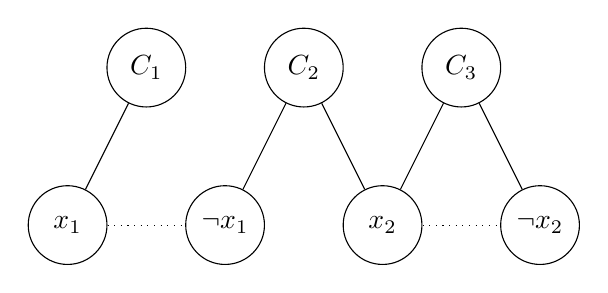
\begin{tikzpicture}[
        every node/.style={draw, circle, minimum size=1cm},
        node distance=1.5cm,
        scale=0.8,
    ]
        % Define Literal Nodes
        \node (x1) at (0, 0) {\(x_1\)};
        \node (notx1) at (2.5, 0) {\(\neg x_1\)};
        \node (x2) at (5, 0) {\(x_2\)};
        \node (notx2) at (7.5, 0) {\(\neg x_2\)};
        
        % Define Clause Nodes (one level above literals)
        \node[circle, draw] (C1) at (1.25, 2.5) {\(C_1\)};
        \node[circle, draw] (C2) at (3.75, 2.5) {\(C_2\)};
        \node[circle, draw] (C3) at (6.25, 2.5) {\(C_3\)};
        
        % Draw Edges (Literal → Clause)
        \draw (x1) -- (C1);
        \draw (notx1) -- (C2);
        \draw (x2) -- (C2);
        \draw (notx2) -- (C3);
        \draw (x2) -- (C3);
        
        % Draw Dotted Edges between each literal and its co mplement
        \draw[dotted] (x1) -- (notx1);
        \draw[dotted] (x2) -- (notx2);
    \end{tikzpicture}
    \caption{LCG representation of $\psi(V)$ with dashed lines representing the connection between complementary literals relevant for the message passing in GNNs.}
    \label{fig:lcg-sat}
\end{figure}

%\subsection{Incidence/Levi graph?}
%Defined in ALYAHYA et al. Concrete graphical representation of SAT? Type of bipartite graph.
%Defines edges via edge weight function! PART OF GRAPH THEORY \\
%Definition in Cimatti et al. : For clause $c$ we use $lit(c)$ and $var(c)$ to reference the %set of literals and variables in $c$ respectively. "$For a CNF formula F we write
%cla(F) for its set of clauses, lit(F)= c \in cla(F) lit(c) for its set of literals, and
%var(F)= c \in cla(F) var(c) for its set of variables.$"  Incidence graph of $\psi$ is the %bipartite graph $inc(\psi) = (V,E)$ with $V=lit(\psi) \cup cla(\psi)$. Additionally for %literal $x \in lit(\psi)$ and clause $c \in cla(\psi)$ we define $xc \in E$ if $x \in var(c)$.

\subsection{Unsatisfiable Cores}
The core of an unsatisfiable formula in CNF is a subset of the formula that is also unsatisfiable. Every unsatisfiable formula therefore is a core on its own, but can be broken down into smaller cores. The smaller a core the more significance it holds. A minimal unsatisfiable core is also referred to as a minimal unsatisfiable subset (MUS). SAT solvers like minisat\cite{een2003extensible} are able to compute unsatisfiable cores but do not generally provide a MUS due to high computational cost. However, several deletion-based algorithms exist for computing MUSs (see Torlak et al.\cite{10.1007/978-3-540-68237-0_23}).